\begin{frame}
  \frametitle{Originators of \texttt{libMesh}}
  \begin{block}{}
    \begin{itemize}
    \item 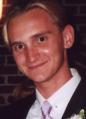
\includegraphics[scale=3]{benkirk} Benjamin S. Kirk, NASA Johnson Space Center
    \item 
\includegraphics[scale=0.35]{jwpeterson} John W. Peterson, Idaho National Lab
    \item 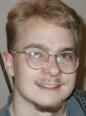
\includegraphics[scale=0.35]{roystgnr} Roy H. Stogner, University of Texas at Austin
    \end{itemize}
  \end{block}

\end{frame}

\frame
{
  \frametitle{Thanks to Dr.\ Graham F.\ Carey}

  \begin{columns}
    \begin{column}{.55\textwidth}
      \scriptsize
      \begin{quote}
        The original development team was heavily influenced by Professor Graham F. Carey, professor of aerospace engineering and engineering mechanics at The University of Texas at Austin, director of the ICES Computational Fluid Dynamics Laboratory, and holder of the Richard B. Curran Chair in Engineering.

        Many of the technologies employed in libMesh were implemented because Dr. Carey taught them to us, we went back to the lab, and immediately began coding. In a very real way, he was ultimately responsible for this library that we hope you may find useful, despite his continued insistence that ``no one ever got a PhD from here for writing a code.''
      \end{quote}
\normalsize
    \end{column}
    \begin{column}{.45\textwidth}
      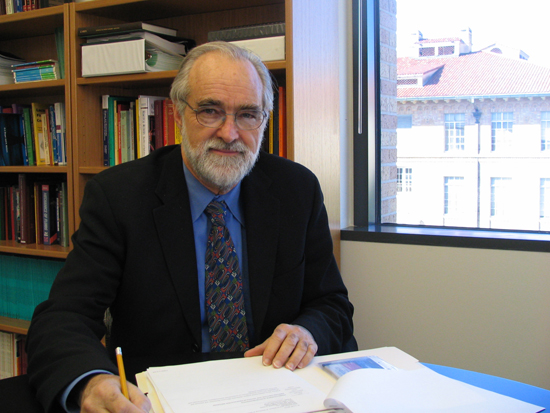
\includegraphics[width=\textwidth]{grahamcarey}
    \end{column}
  \end{columns}
}

% The optional argument [<+->] means everything on the frame will be displayed incrementally.


\begin{frame}[shrink]
  \begin{block}{Code Contributors}
    \scriptsize
    \begin{center}
      \begin{tabular}{|l|l|} \hline
        Benjamin S. Kirk & benkirk \\
        Bill Barth       & bbarth \\
        Cody Permann     & permcody \\
        Daniel Dreyer    & ddreyer \\
        David Andrs      & andrsd \\
        David Knezevic   & knezed01 \\
        Derek Gaston     & friedmud \\
        Dmitry Karpeev   & karpeev \\
        Florian Prill    & fprill \\
        Jason Hales      & jasondhales \\
        John W. Peterson & jwpeterson \\
        Paul T. Bauman   & pbauman \\
        Roy H. Stogner   & roystgnr \\
        Steffen Petersen & spetersen \\
        Sylvain Vallaghe & svallagh \\
        Tim Kroeger      & sheep\_tk \\
        Truman Ellis     & trumanellis \\
        Wout Ruijter     & woutruijter \\ \hline
      \end{tabular}
    \end{center}
    \begin{itemize}
      \item Thanks to Wolfgang Bangerth and the \texttt{deal.II} team for initial technical inspiration.
      \item Also, thanks to Jed Brown, Robert McLay, \& many others for discussions over the years.
    \end{itemize}
  \end{block}
\end{frame}
